\section{Verification and Validation} \label{sec:verificationAndValidation}



% -------------------------------------------------------------------------------
\subsection{Flat plate boundary layer} \label{sec:flatPlateBoundaryLayer}


In this section we consider the computation of the flow over a flat plate.
The plate is horizontal and starts at $(x,y)=(0,0)$.
The boundary layer solution is an approximation solution to the laminar flow past a flat plate. The
solution  is given by (derived by Prandtl's student Blasius)
\begin{align*}
   & u = U f'(\eta), \\
   & v = \half \sqrt{\frac{\nu U}{x}} \Big( \eta f' - f \Big), 
\end{align*}
where the similiarity variable $\eta$ is defined as
\begin{align*}
   & \eta = y\, \sqrt{\frac{U}{\nu x}},
\end{align*}
and where $f$ satisfies the 3rd order ODE:
\begin{align*}
   & f f'' + 2 f ''' = 0, \qquad f(0)=0, ~ f'(0)=0, ~ f'(\infty)=1.
\end{align*}
This problem can be solved as a shooting problem with initial condition
\begin{align*}
   f''(0) \approx 0.3320573362151946
\end{align*}
Note that $v$ only makes sense if $\sqrt{\frac{\nu U}{x}}$ is small which implies $\nu$ is small
and $x$ is not too small (i.e. we cannot evaluate the solution too close to the leading edge). 
We thus start the computation at some offset value $x=x_0$

The thickness of the boundary layer is
\begin{align*}
   \delta(x) \approx C_\delta \sqrt{\frac{\nu x}{U}} , 
\end{align*}
where $C_\delta\approx 5$ for $u\approx .99 U$ on the edge of the boundary layer. 
The thickness of the boundary layer at inflow will this be $\delta(x_0)$ and we should therefore have
enough grid points to resolve this layer. 

This boundary solution is evaluated in the class {\tt BoundaryLayerProfile}.
Since the solution is only approximate the errors will not go zero as the mesh is refined.
The errors should become smaller, however, as $\sqrt{\frac{\nu U}{x_0}} \rightarrow 0$, e.g. 
if $\nu\rightarrow 0$ or $x_0\rightarrow\infty$. 


The cgins script {\tt flatPlate.cmd} can be used to solve for the flow past a flat plate.

Figure~\ref{fig:boundaryLayer} shows results for the flat plate boundary layer.

{
\newcommand{\figWidthp}{8.cm}
\newcommand{\trimfig}[2]{\trimPlotb{#1}{#2}{.0}{.0}{.0}{.0}}
\begin{figure}[hbt]
\begin{center}
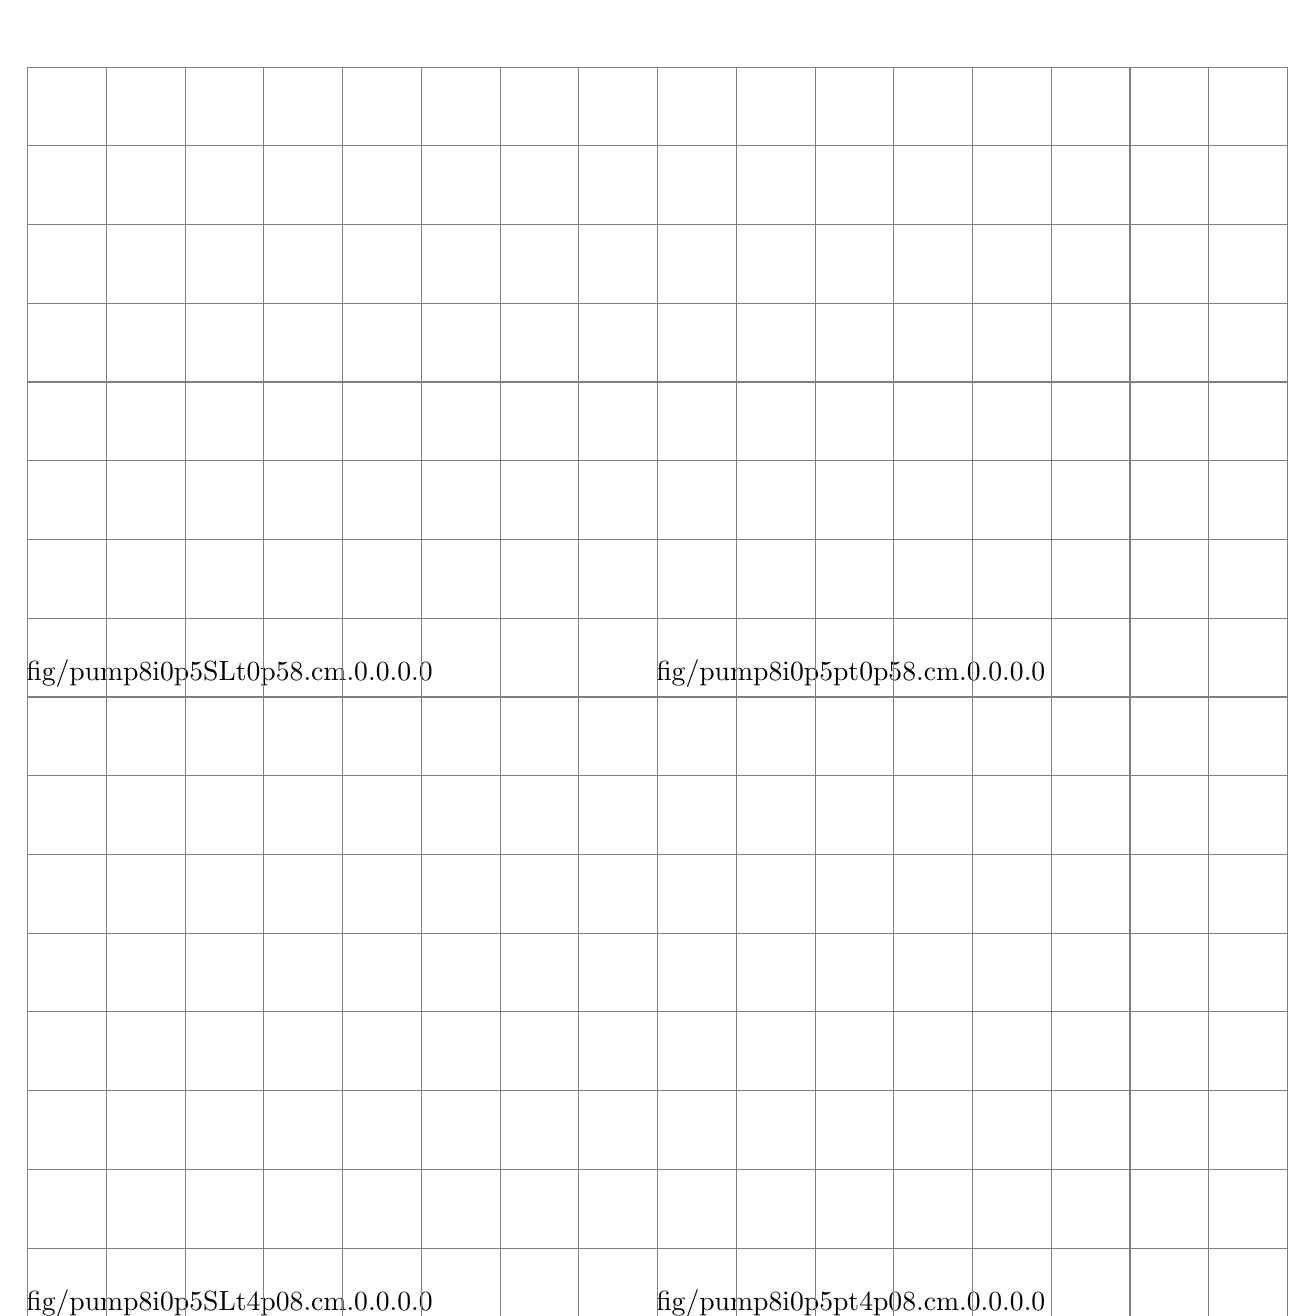
\begin{tikzpicture}[scale=1]
  \useasboundingbox (0,.5) rectangle (16.,16.5);  % set the bounding box (so we have less surrounding white space)
%
  \draw ( 0.0, 8) node[anchor=south west,xshift=-4pt,yshift=+0pt] {\trimfig{fig/pump8i0p5SLt0p5}{\figWidthp}};
  \draw ( 8.0, 8) node[anchor=south west,xshift=-4pt,yshift=+0pt] {\trimfig{fig/pump8i0p5pt0p5}{\figWidthp}};
  \draw ( 0.0, 0) node[anchor=south west,xshift=-4pt,yshift=+0pt] {\trimfig{fig/pump8i0p5SLt4p0}{\figWidthp}};
  \draw ( 8.0, 0) node[anchor=south west,xshift=-4pt,yshift=+0pt] {\trimfig{fig/pump8i0p5pt4p0}{\figWidthp}};
 % \draw (current bounding box.south west) rectangle (current bounding box.north east);
% grid:
 \draw[step=1cm,gray] (0,0) grid (16,16);
\end{tikzpicture}
\end{center}
  \caption{Flat plate boundary layer. }
  \label{fig:boundaryLayer}
\end{figure}
}



% -------------------------------------------------------------------------------
\clearpage
\subsection{Heat transfer verificiation and validation} \label{sec:heatTransferVerificationAndValidation}


In this section we consider some verificiation and validation of the heat transfer capabilities.


%-------------------------------------------------------------------------------
\subsubsection{Heated domain with no flow} \label{sec:heatedBox}

 We consider heat transfer in a domain with no fluid flow. The governing equation is
thus the heat equation for the temperature,
\begin{align}
    T_t &= \kappa \Delta T + f_T, 
\end{align}
where $f_T$ is the body force and $\kappa=k/(\rho C_p)$ is the thermal diffusivity.


\paragraph{Case: heated strip:} One-dimensional heat transfer in a periodic strip with a constant body force heating, 
\begin{align}
   & T_t = \kappa T_{xx} + f_0 , \quad x\in(0,1), \\
   & T(0,y,t)=0, \quad  T(1,y,t)=0, \\
   & T(x,y,t)=T(x,y+1,t), \quad \text{(periodic in y)}, \\
   & T(x,y,0)=0.
\end{align}
The steady state solution is
\begin{align}
    T_p(x) &= \frac{f_0}{2 \kappa} x (1-x ), 
\end{align}
with heat flux on the walls,
\begin{align}
   \Hc =  k T_n = - \frac{f_0}{2}\frac{k}{\kappa} = - \frac{f_0}{2} \rho C_p, \qquad \text{(steady state heat flux at $x=0$ and $x=1$)}.
\end{align}

The solution to the time dependent problem is 
\begin{align}
    T &= T_p(x) + \sum_{n=1}^\infty a_n e^{-\kappa (n\pi)^2 t} \sin(n\pi x), \label{eq:squareHeatSolution} \\
    a_n &= -2 \int_0^1 T_p(x) \sin(n\pi x) dx. 
\end{align}


We solve the problem on a square grid for $[0,1]\times[0,1]$, periodic in the y-direction.
The grid is created with
\begin{flushleft}\tt\small
  ogen -noplot squareArg -periodic=np -order=2 -nx=32
\end{flushleft}
Cgins is run with the command (scheme IM2)
\begin{flushleft}\tt\small
  cgins heatFlux -g=square32np.order2 -nu=.72 -tp=.5 -adcBoussinesq=0. -thermalConductivity=.1 -gravity="0. 0. 0." -go=halt
\end{flushleft}
where $f_0=1$, $k=.1$, $\kappa=1$.

At $t=10$ the peak temperature is $.125000$ (exact is $.125$) and the measured heat flux on the left wall is $\Hc = -4.999778677e-02$ (compared
to the exact value of $\Hc$ = -5e-2). The numerical solution should converge in time to the exact steady-state solution since the 
steady state solution is a polynomial of degree 2.

Fourth-order: 
\begin{flushleft}\tt\small
  ogen -noplot squareArg -periodic=np -order=4 -nx=32 -numGhost=3
\end{flushleft}
Cgins is run with the command (scheme PC24)
\begin{flushleft}\tt\small
  cgins heatFlux -g=square32np.order4.ng3 -nu=.72 -ts=pc -tp=.5 -adcBoussinesq=0. -thermalConductivity=.1 -gravity="0. 0. 0." -go=halt
\end{flushleft}
At $t=2.5$ the heat flux at the wall is $\Hc = -5.000000000e-02$. (Note that $e^{-2.5 \pi^2}\approx 1.9e-11$ so that the time-dependent
part of~\eqref{eq:squareHeatSolution} is small).


\paragraph{Case: heated square:} Two-dimensional heat transfer in the unit square with a body forcing,
\begin{align}
  &  f_T = f_0 \sin(m_x\pi x)\sin(m_y \pi y)  , \\
  &  T(x,y,0) = 0 , 
\end{align}
has solution
\begin{align}
    T(x,y,t) &= \frac{f_0}{\alpha} ( 1 - e^{-\alpha t}) \sin(m_x\pi x)\sin(m_y \pi y)  , \\
    \alpha &= ( m_x^2 + m_y^2 ) \pi^2 \kappa. 
\end{align}

The average temperature in the 2D domain $[0,1]^2$ is 
\begin{align}
    \bar{T} &=
  \begin{cases} 
 \frac{f_0}{\alpha} ( 1 - e^{-\alpha t}) ~ \frac{2}{m_x \pi}~ \frac{2}{m_y \pi},  & \text{for $m_x$ odd and $m_y$ odd},\\
            0 , &  \text{otherwise} 
  \end{cases} .
\end{align}
The average heat flux on $x=0$ is
\begin{align}
   \Hc(x=0) & = \int_0^1 -k T_x dy = -k ( 1 - e^{-\alpha t}) \int_0^1 m_x \pi \cos(m_x\pi x) \sin(m_y \pi y) dy \\
            &= 
          \begin{cases} 
            - k( 1 - e^{-\alpha t}) ~ \frac{2 m_x}{m_y} , & \text{for $m_y$ odd},\\
            0 , & \text{for $m_y$ even}.
          \end{cases} .
\end{align}

Solving this problem with Cgins on grid {\tt square32.order2} to steady state ($\nu=.72$, $\kappa=1$, $k=.1$) gives a 
peak temperature of $T_{\max}=1.000804$ (true value $T_{\max}=1$), the average (integrated) temperature of $\bar{T}=.4050$ (true value 
$\bar{T}=(2/\pi)^2\approx .4052847$) and the average (summed not integrated -- fix me) heat flux of $\Hc(x=0)=-.1946$ (true value $\Hc(0)=-.2$).


\paragraph{Case: heated box:} Three-dimensional heat transfer in the unit square with a body forcing,
\begin{align}
  &  f_T = f_0 \sin(m_x\pi x)\sin(m_y \pi y)\sin(m_z \pi z)  , \\
  &  T(x,y,z,0) = 0 , 
\end{align}
has solution
\begin{align}
    T(x,y,t) &= \frac{f_0}{\alpha} ( 1 - e^{-\alpha t}) \sin(m_x\pi x)\sin(m_y \pi y)\sin(m_z \pi z)  , \\
    \alpha &= ( m_x^2 + m_y^2 + m_z^2) \pi^2 \kappa. 
\end{align}
The average temperature in the 3D domain $[0,1]^3$ is 
\begin{align}
    \bar{T} &=
  \begin{cases} 
   \frac{f_0}{\alpha} ( 1 - e^{-\alpha t}) ~ \frac{2}{m_x \pi}~ \frac{2}{m_y \pi}~ \frac{2}{m_z \pi} & 
                      \text{for $m_x$ odd and $m_y$ odd and $m_zy$ odd},\\
            0 , &  \text{otherwise} 
  \end{cases} .
\end{align}
The average heat flux on the face $x=0$ is
\begin{alignat}{3}
   \Hc(x=0) & = \int_0^1\int_0^1 -k T_x dy dz \\
            & = -k ( 1 - e^{-\alpha t}) \int_0^1 \int_0^1 -k m_x \pi \cos(m_x\pi x) \sin(m_y \pi y)sin(m_z \pi z) dy dz\\
       &= 
          \begin{cases} 
            - k( 1 - e^{-\alpha t}) ~ \frac{4 m_x}{\pi m_y m_z} , & \text{for $m_y$ odd and $m_z$ odd},\\
            0 , & \text{for $m_y$ even}.
          \end{cases} .
\end{alignat}
%            T : (min,max)=( 0.000000e+00, 1.000804e+00)
% probeRegion pr=0: t=2.000e+00, average = -1.200e-01
% probeRegion pr=1: t=2.000e+00, average = -1.200e-01
% probeRegion pr=2: t=2.000e+00, average = 2.576e-01
Solving this problem with Cgins on grid {\tt box32.order2} to steady state ($\nu=.72$, $\kappa=1$, $k=.1$) gives a 
peak temperature of $T_{\max}=1.000804$ (true value $T_{\max}=1$), the average (integrated) temperature of $\bar{T}=.2576$ (true value 
$\bar{T}=(2/\pi)^3\approx .258012$) and the average (summed not integrated -- fix me) heat flux of $\Hc(x=0)=-.120$ (true value $\Hc(0)=-.127324$).


\paragraph{Case: steady heated box:} Steady state heating of a box. If we choose a constant source
of heat in the sub-region $\Rc=[.5(1-d),.5(1+d)]^3$ (i.e. a sub-cube of width $d$ in each direction and volume $d^3$) of the unit box $[0,1]^3$,
\begin{align}
    f_T = f_0 , \quad \text{for $\xv\in \Rc$}, 
\end{align}
then in steady state the total heat flux through the boundary will be
\begin{align}
    \int_{\partial\Bc} k T_n dS &= - \frac{k}{\kappa} \int_{\Bc} f_T d\xv , \\
                                &= - \frac{k}{\kappa} f_0 d^3 . 
\end{align}
